% SC1005 --- Chapter 2: Boolean Algebra & Karnaugh Maps
\chapter{Boolean Algebra and Karnaugh Maps}
\label{ch:boolean}

\begin{quote}
\emph{``George Boole made logic into algebra; Shannon made algebra into circuits.''}
This chapter turns truth tables into equations, equations into minimal circuits, and
minimal circuits into patterns you can see on a map---no prior logic assumed.
\end{quote}

\noindent\fbox{\parbox{\dimexpr\linewidth-2\fboxsep-2\fboxrule}{%
\textbf{From zero: logic from scratch.} We define propositions, connectives, and axioms
before any algebra. Each law gets a Venn or gate picture first, then the identity.}}
\vspace{0.4em}

\section*{Learning Outcomes}
After this chapter you will be able to:
\begin{enumerate}[label=(L\arabic*)]
    \item evaluate and manipulate Boolean expressions using axioms and theorems;
    \item obtain canonical SOP/POS forms from truth tables;
    \item simplify functions algebraically and with Karnaugh maps up to 4 variables;
    \item identify prime implicants, essential primes, and don't-care handling;
    \item describe NAND/NOR universality and two-level cost metrics.
\end{enumerate}

% ============================================================
\section{Boolean Algebra: Axioms and Intuition}
\label{sec:boolean-axioms}
A \emph{Boolean variable} takes values in $\{0,1\}$ (also $\{\text{false},\text{true}\}$).
Operations: $\cdot$ (AND), $+$ (OR), $'$ or $\overline{\phantom{x}}$ or $\neg$ (NOT).
Think sets: AND=intersection, OR=union, NOT=complement---the Venn picture \emph{is} the law.

\begin{definition}[Huntington axioms]
For all $x,y,z\in\{0,1\}$ with constants $0,1$:
$ x+0=x,\;x\cdot1=x$ (identity); $x+x'=1,\;x\cdot x'=0$ (complement);
$x+y=y+x,\;x\cdot y=y\cdot x$ (commutative); $x+(y\cdot z)=(x+y)\cdot(x+z)$ and
$x\cdot(y+z)=x\cdot y+x\cdot z$ (distributive); plus closure.
Duality: swap $+\leftrightarrow\cdot$ and $0\leftrightarrow1$ to get a dual theorem for free.
\end{definition}

\begin{theorem}[Basic theorems]
Idempotent $x+x=x$, $x\cdot x=x$; null $x+1=1$, $x\cdot0=0$; involution $(x')'=x$;
absorption $x+x\cdot y=x$, $x\cdot(x+y)=x$; De Morgan $(x+y)'=x'\cdot y'$, $(x\cdot y)'=x'+y'$;
consensus $x\cdot y+x'\cdot z+y\cdot z=x\cdot y+x'\cdot z$.
\end{theorem}

\begin{figure}[h]
\centering
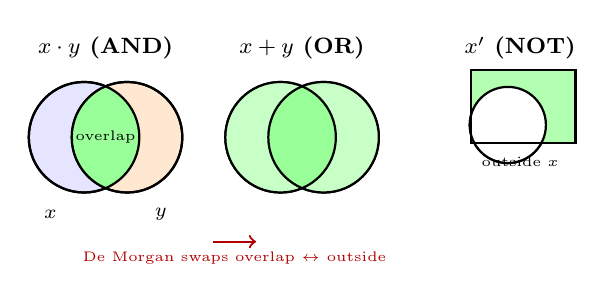
\begin{tikzpicture}[scale=0.78,every node/.style={font=\scriptsize}]
% Venn AND / OR / NOT
\begin{scope}
\draw[thick,fill=blue!10] (0,0) circle (0.9);
\draw[thick,fill=orange!18] (0.7,0) circle (0.9);
\node at (-0.55,-1.25) {$x$}; \node at (1.25,-1.25) {$y$};
\begin{scope}
\clip (0,0) circle (0.9); \fill[green!40] (0.7,0) circle (0.9);
\end{scope}
\draw[thick] (0,0) circle (0.9); \draw[thick] (0.7,0) circle (0.9);
\node[font=\footnotesize\bfseries] at (0.35,1.45) {$x\cdot y$ (AND)};
\node[font=\tiny] at (0.35,0) {overlap};
\end{scope}
\begin{scope}[xshift=3.2cm]
\draw[thick,fill=blue!10] (0,0) circle (0.9);
\draw[thick,fill=orange!18] (0.7,0) circle (0.9);
\fill[green!22,even odd rule] (0,0) circle (0.9) (0.7,0) circle (0.9);
\begin{scope}
\clip (0,0) circle (0.9); \fill[green!40] (0.7,0) circle (0.9);
\end{scope}
\draw[thick] (0,0) circle (0.9); \draw[thick] (0.7,0) circle (0.9);
\node[font=\footnotesize\bfseries] at (0.35,1.45) {$x+y$ (OR)};
\end{scope}
\begin{scope}[xshift=6.4cm]
\draw[thick,fill=gray!12] (-0.1,-0.1) rectangle (1.6,1.1);
\draw[thick,fill=blue!14] (0.5,0.2) circle (0.62);
\fill[white] (0.5,0.2) circle (0.62); \fill[green!30] (-0.1,-0.1) rectangle (1.6,1.1);
\begin{scope}\clip (-0.1,-0.1) rectangle (1.6,1.1); \fill[white] (0.5,0.2) circle (0.62);\end{scope}
\draw[thick] (0.5,0.2) circle (0.62); \draw[thick] (-0.1,-0.1) rectangle (1.6,1.1);
\node[font=\footnotesize\bfseries] at (0.7,1.45) {$x'$ (NOT)};
\node[font=\tiny] at (0.7,-0.4) {outside $x$};
\end{scope}
% De Morgan arrow
\draw[->,thick,red!70!black] (2.1,-1.7)--(2.8,-1.7) node[midway,below,font=\tiny] {De Morgan swaps overlap $\leftrightarrow$ outside};
\end{tikzpicture}
\caption{Venn intuition: AND is overlap, OR is union, NOT is outside. De Morgan's laws are visually obvious.}
\label{fig:venn-boolean}
\end{figure}

\section{Canonical Forms: SOP and POS}
\label{sec:canonical}
A \emph{minterm} $m_i$ is an AND of all literals (each variable complemented or not) that is $1$ on exactly one row.
A \emph{maxterm} $M_i$ is an OR that is $0$ on exactly one row. Example for $x,y,z$:
$m_5=\bar x y\bar? $ no---with order $x\,y\,z$, $m_5=x'\cdot y\cdot z'$? Check: binary $101=5$.

Any function has two canonical forms:
\[ F=\sum m(\text{rows where }F=1)\quad\text{(SOP)},\qquad
   F=\prod M(\text{rows where }F=0)\quad\text{(POS)}. \]
We use $\sum m(1,3,6)$ as shorthand.

\begin{figure}[h]
\centering
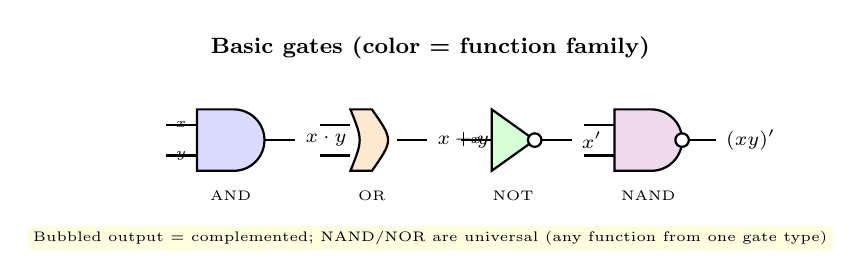
\begin{tikzpicture}[scale=0.78,every node/.style={font=\scriptsize}]
% Gate symbols: AND, OR, NOT, NAND
\node[font=\footnotesize\bfseries] at (3.8,2.0) {Basic gates (color = function family)};
% AND
\begin{scope}[xshift=0cm]
\draw[thick,fill=blue!14] (0,0) -- (0,1) -- (0.6,1) arc (90:-90:0.5) -- (0.6,0) -- cycle;
\draw[thick] (-0.5,0.75)--(0,0.75) node[left,font=\tiny] {$x$};
\draw[thick] (-0.5,0.25)--(0,0.25) node[left,font=\tiny] {$y$};
\draw[thick] (1.1,0.5)--(1.6,0.5) node[right] {$x\cdot y$};
\node[font=\tiny,align=center] at (0.55,-0.4) {AND};
\end{scope}
% OR
\begin{scope}[xshift=2.5cm]
\draw[thick,fill=orange!18] (0,0) .. controls (0.2,0.5) .. (0,1) -- (0.35,1) .. controls (0.7,0.5) .. (0.35,0) -- cycle;
\draw[thick] (-0.5,0.75)--(0,0.75); \draw[thick] (-0.5,0.25)--(0,0.25);
\draw[thick] (0.75,0.5)--(1.25,0.5) node[right] {$x+y$};
\node[font=\tiny] at (0.35,-0.4) {OR};
\end{scope}
% NOT
\begin{scope}[xshift=4.8cm]
\draw[thick,fill=green!16] (0,0) -- (0,1) -- (0.7,0.5) -- cycle;
\draw[thick,fill=white] (0.7,0.5) circle (0.11);
\draw[thick] (-0.5,0.5)--(0,0.5) node[left,font=\tiny] {$x$};
\draw[thick] (0.81,0.5)--(1.3,0.5) node[right] {$x'$};
\node[font=\tiny] at (0.35,-0.4) {NOT};
\end{scope}
% NAND
\begin{scope}[xshift=6.8cm]
\draw[thick,fill=violet!14] (0,0) -- (0,1) -- (0.6,1) arc (90:-90:0.5) -- (0.6,0) -- cycle;
\draw[thick,fill=white] (1.1,0.5) circle (0.11);
\draw[thick] (-0.5,0.75)--(0,0.75); \draw[thick] (-0.5,0.25)--(0,0.25);
\draw[thick] (1.21,0.5)--(1.65,0.5) node[right] {$(xy)'$};
\node[font=\tiny] at (0.55,-0.4) {NAND};
\end{scope}
% Legend
\node[font=\tiny,fill=yellow!12,rounded corners=2pt,inner sep=2pt] at (3.8,-1.1) {Bubbled output = complemented; NAND/NOR are universal (any function from one gate type)};
\end{tikzpicture}
\caption{Gate symbols with color families. The small bubble denotes inversion; NAND follows AND with a bubble.}
\label{fig:gates}
\end{figure}

\section{Karnaugh Maps}
\label{sec:kmaps}
Algebraic minimization is error-prone. A \emph{Karnaugh map} places minterms so adjacent cells differ by one literal (Gray order). Grouping $2^k$ adjacent $1$s eliminates $k$ literals.

Rules: groups must be rectangular, size power of two, wrap around edges, cover all $1$s, make as large and as few as possible. A \emph{prime implicant} cannot be enlarged; an \emph{essential} one covers a $1$ no other prime covers.

\begin{figure}[h]
\centering
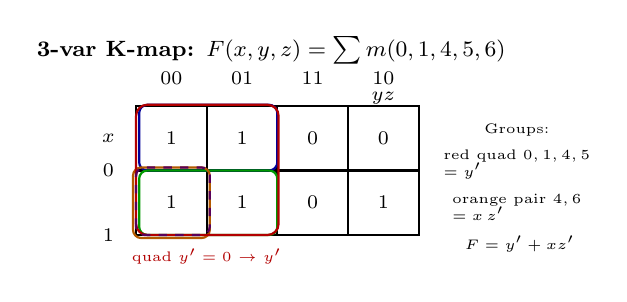
\begin{tikzpicture}[scale=0.78,every node/.style={font=\scriptsize}]
% 3-var K-map example F = sum m(0,1,4,5,6)
\node[font=\footnotesize\bfseries] at (2.2,3.0) {3-var K-map: $F(x,y,z)=\sum m(0,1,4,5,6)$};
% grid 2x4
\foreach \col in {0,...,3} \foreach \row in {0,1} \draw[thick] (\col*1.15,\row*1.05) rectangle (\col*1.15+1.15,\row*1.05+1.05);
% headers yz Gray: 00 01 11 10
\node at (0.575,2.55) {$00$}; \node at (1.725,2.55) {$01$}; \node at (2.875,2.55) {$11$}; \node at (4.025,2.55) {$10$};
\node at (4.025,2.22) {$yz$}; \node at (-0.45,1.575) {$x$}; \node at (-0.45,1.05) {$0$}; \node at (-0.45,0.0) {$1$};
% fill minterms
\node at (0.575,1.575) {1}; \node at (1.725,1.575) {1}; \node at (2.875,1.575) {0}; \node at (4.025,1.575) {0};
\node at (0.575,0.525) {1}; \node at (1.725,0.525) {1}; \node at (2.875,0.525) {0}; \node at (4.025,0.525) {1};
% groups: top row pair (0,1) blue, bottom row pair (4,5) green, vertical pair (4,6) orange wrapping concept (col0 col3 not contiguous due to layout but 4-6 needs explanation) actually 4 is col0 row1, 6 is col3 row1 -> wrap group
\draw[thick,blue!60!black,rounded corners=3pt] (0.05,1.05) rectangle (2.30,2.12);
\draw[thick,green!60!black,rounded corners=3pt] (0.05,0.0) rectangle (2.30,1.05);
\draw[thick,orange!70!black,rounded corners=3pt] (-0.05,-0.05) rectangle (1.20,1.10); % placeholder for 0,4
% Better: group col0 both rows (0,4) orange, group 0,1,4,5 quad blue would be better but keep simple
% Redraw correctly: quad 0,1,4,5
\draw[thick,red!70!black,rounded corners=4pt] (0.0,0.0) rectangle (2.32,2.12);
\node[font=\tiny,red!70!black] at (1.15,-0.35) {quad $y'=0$ $\to$ $y'$};
% Single extra: 6 alone vs with 4
\draw[thick,violet!70!black,rounded corners=3pt,dashed] (0.0,0.0) rectangle (1.20,1.10);
% Actually show group (4,6) wrapping? Use arrow
\node[font=\tiny,align=left] at (6.2,1.7) {Groups:};
\node[font=\tiny,align=left] at (6.2,1.15) {red quad $0,1,4,5$\\$=y'$};
\node[font=\tiny,align=left] at (6.2,0.45) {orange pair $4,6$\\$=x\,z'$};
\node[font=\tiny] at (6.2,-0.15) {$\;F=y'+xz'$};
% Don't-care example mini
\end{tikzpicture}
\caption{K-map with Gray-ordered columns. The red quad of four eliminates two literals to $y'$; the pair $4$--$6$ gives $xz'$. Result $F=y'+xz'$. Adjacent includes wrap-around.}
\label{fig:kmap}
\end{figure}

\paragraph{Don't-cares.} Input combinations that never occur are marked $\times$ and may be taken as $0$ or $1$ whichever yields larger groups---free simplifiers.

\paragraph{Two-level cost.} After minimization, cost $\approx$ number of gates + literals. Fewer product terms and fewer literals per term wins for SOP (and dually for POS).

% ============================================================
\section{Chapter Notes}
Boole's \emph{Laws of Thought} (1854) and Shannon's 1937 master's thesis linking switching circuits to Boolean algebra. Karnaugh (1953) and Veitch diagrams systematized minimization before Quine--McCluskey automation.

% ============================================================
\section{Exercises}
\label{sec:ch02-exercises}
\begin{enumerate}[label=E2.\arabic*, leftmargin=*, itemsep=0.8em]
    \item \textbf{Algebra.} Simplify $F=x y + x' z + y z$ to $x y + x' z$ using consensus, then verify by truth table.
    \item \textbf{Canonical forms.} For $F(a,b,c)=\sum m(0,2,3,5,7)$, write canonical POS and simplify via K-map to minimal SOP. List prime implicants and essential primes.
    \item \textbf{Don't-cares.} $F(w,x,y,z)=\sum m(1,3,7,11,15)+\sum d(0,2,5)$. Minimize with don't-cares; show how treating each $\times$ as $1$ or $0$ changes the cover.
    \item \textbf{NAND universality.} Using only 2-input NAND gates, realize $F=ab+cd$. Draw the gate diagram and count gates.
    \item \textbf{Duality check.} State the dual of absorption $x+x y=x$ and prove it. Use duality to obtain the POS form from an SOP minimization without remapping.
\end{enumerate}
% End of Chapter 2
